\usepackage[authoryear,round]{natbib}
\usepackage{multirow}

\newcommand{\sheetnum}{%
	00
}
%\setcounter{section}{\sheetnum-3}
\newcommand{\tutorialtitle}{%
    Introduction \& Method of Lagrange Multipliers
}
\newcommand{\tutorialtitleshort}{%
	Intro \& Lagrange
}
% for slides
\subtitle{\sheetnum \tutorialtitle}

%\maxdeadcycles=1000 % Workaround for ! Output loop---100 consecutive dead cycles because of too many figures

% The following use of algroithms does not work well with the notes:
%
%
%
%
% instead use the following for your algorithms:
%
%\begin{figure}[!t]
%\removelatexerror
%\begin{algorithm}[H]
    % your algo here
    %\label{alg:algolabel}
    %\caption{algocaption}
%\end{algorithm}
%\end{figure}
%\begin{algorithm}
% Below is the definition for the command \removelatexerror:
\makeatletter
\newcommand{\removelatexerror}{\let\@latex@error\@gobble}
\makeatother

\begin{document} %%%%%%%%%%%%%%%%%%%%%%%%%%%%%%%%%%%%%%%%%%%%%%%%%%%%%%%

\sheet{\sheetnum}{\tutorialtitleshort}

\ttopic{\tutorialtitle}

\columnratio{0.2,0.8}\textbf{}
\begin{paracol}{2}
%\setlength{\columnseprule}{0.1pt}
%\setlength{\columnsep}{5em}

\begin{rightcolumn}

% notes version will ignore it
\begin{frame}
\titlepage
\end{frame}

\begin{frame}
\tableofcontents
\end{frame}

\newpage

\mode<all>
\section{Introduction}

\definecolor{darkgreen}{rgb}{0,0.6,0}

\mode<presentation>{
\begin{frame}
    \begin{center}
    \slidesonly{\huge}\secname
    \end{center}
    \begin{center}
        What to expect
        and not to expect
        from this course
    \end{center}
    \pause
\end{frame}
}

\subsection{Learning Paradigms}

\subsubsection{Supervised learning}

\begin{frame}{\subsecname:~\subsubsecname}

We are given data that is made up of tuples.

Supervised methods try to fit a function that maps $\vec x$ to some attribute $\vec y$ (labels/ground truth).

\begin{center}
	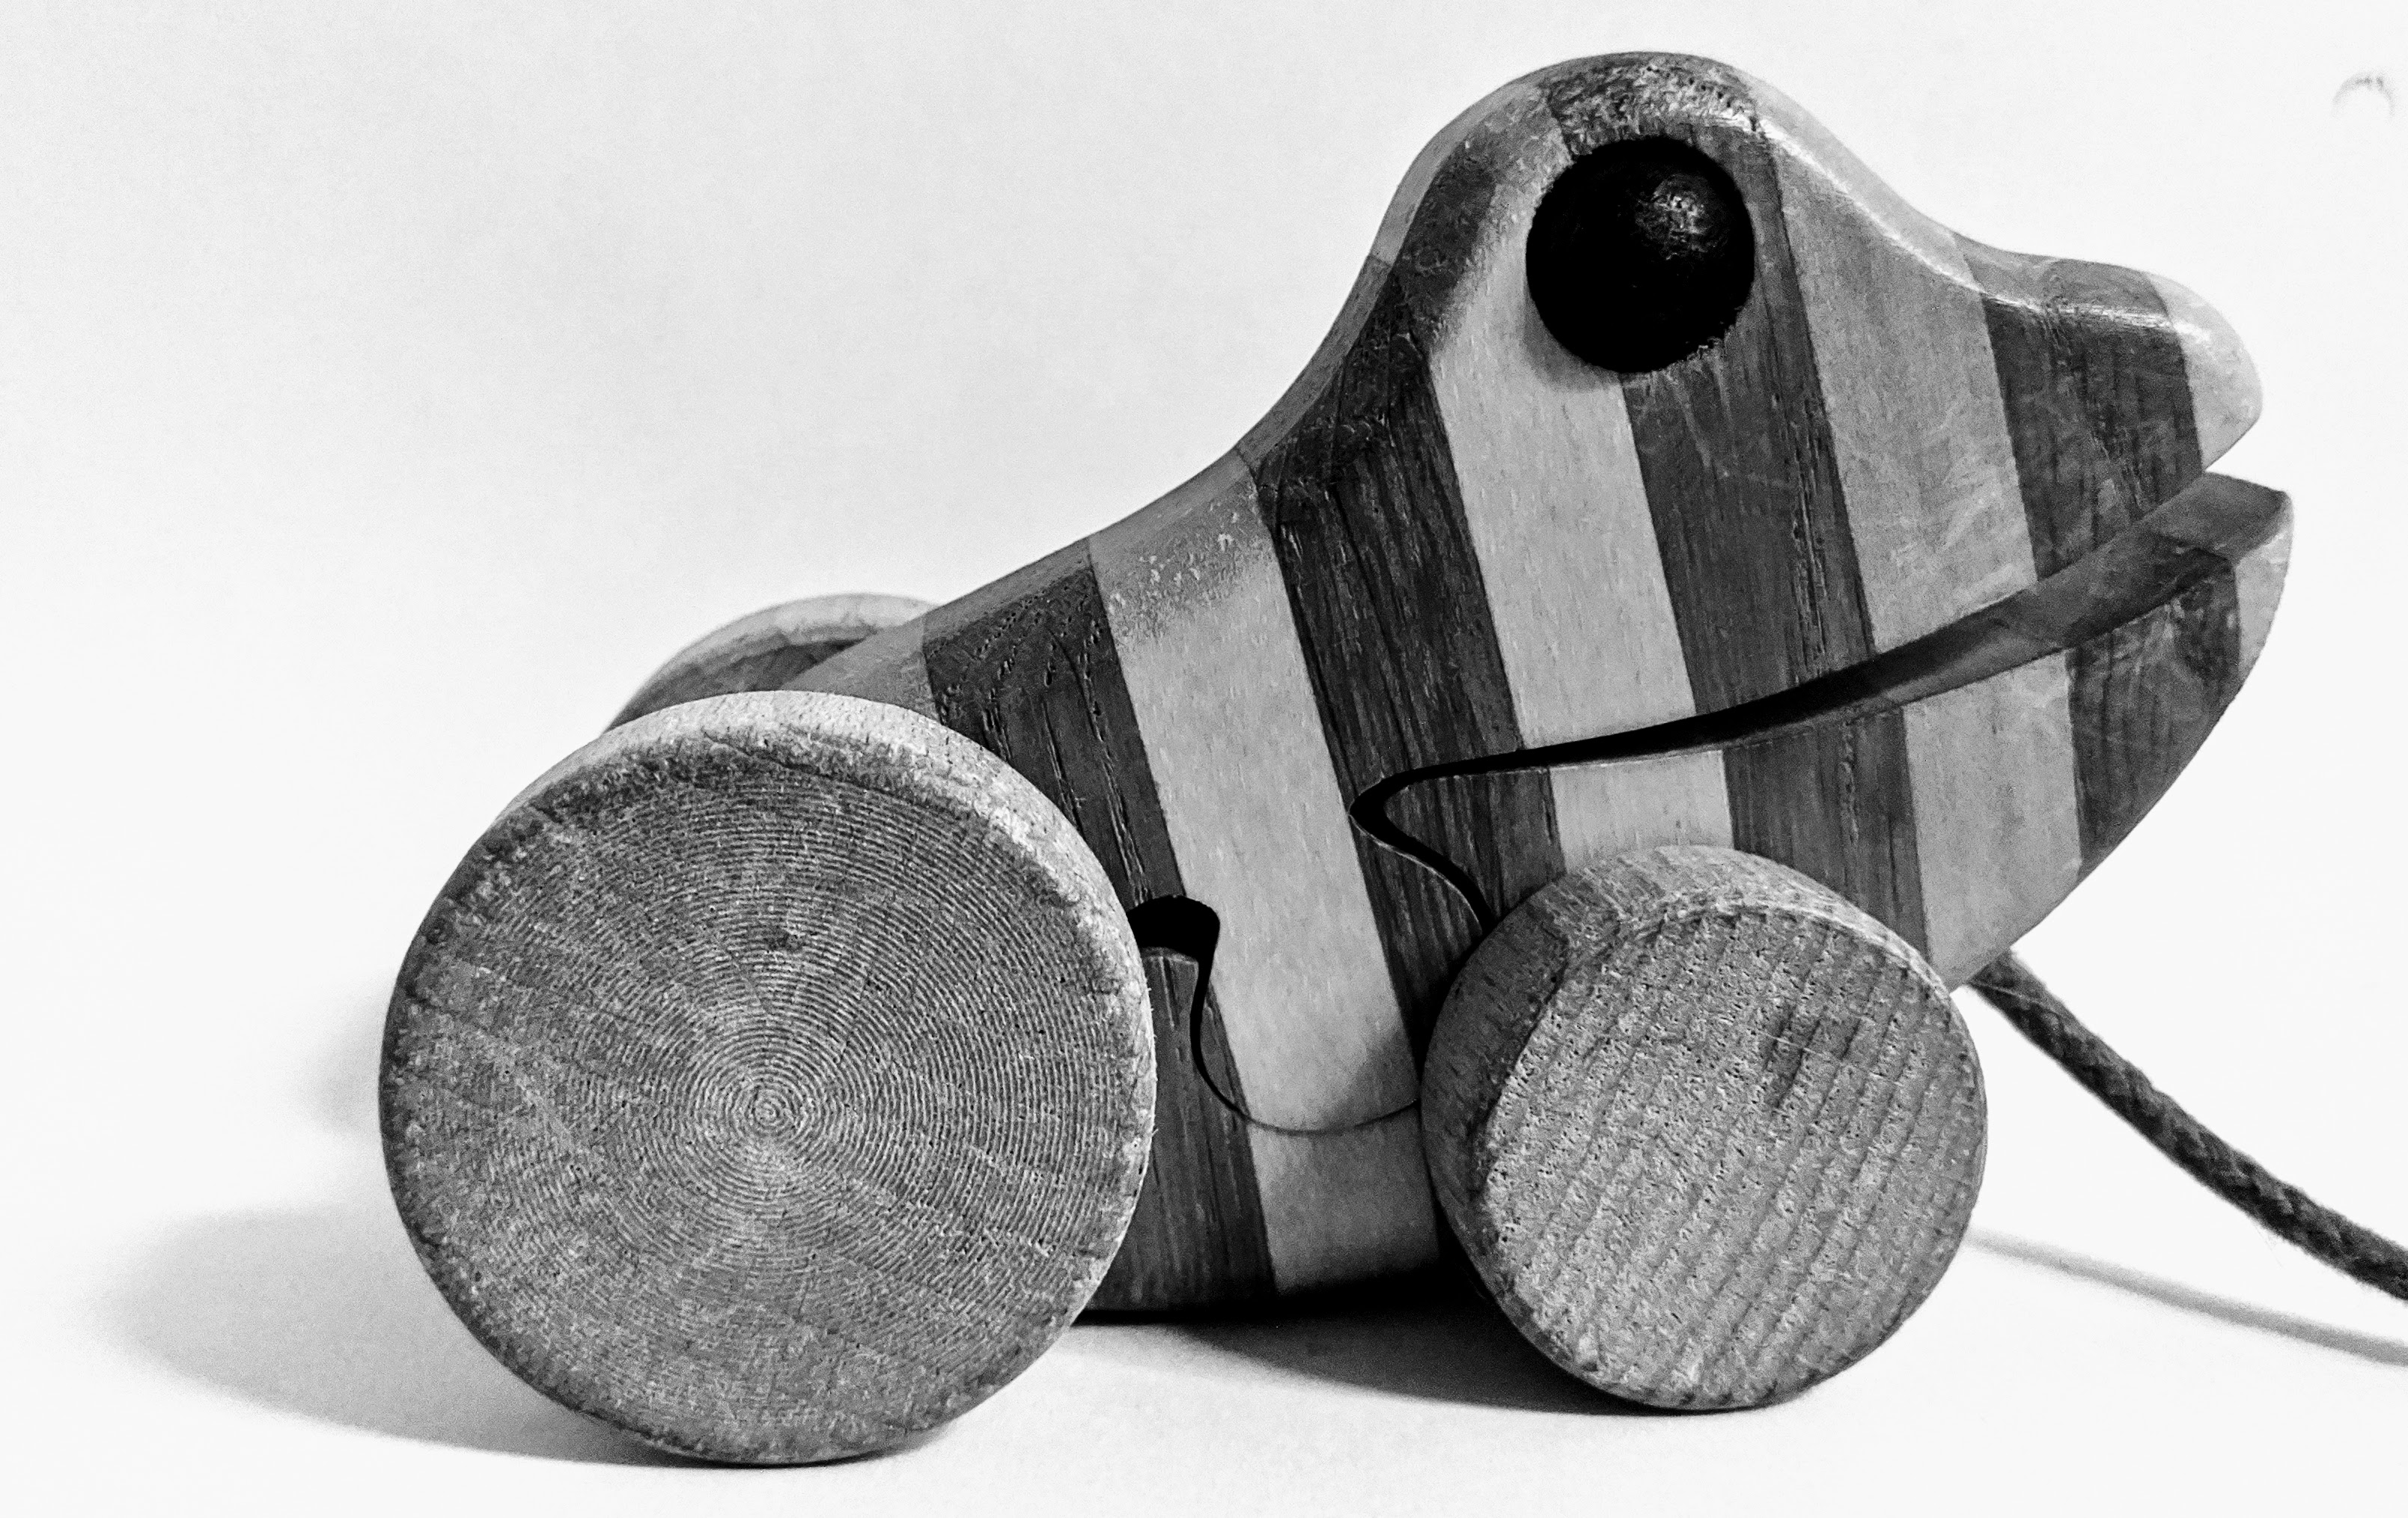
\includegraphics[height=3cm]{img/tigerente}
	\captionof*{figure}{example image recognition}
\end{center}

Supervised learning would fit a function that maps image pixels to recognizing the object in the image\\
from a set of possible objects (e.g. cat, dog, tiger, duck, frog, bird).
    
\end{frame}

\subsubsection{Unsupervised learning}

\begin{frame}{\subsecname: \subsubsecname}

We are given data that is made up of observations\pause~\textbf{only}. No other information.

\mode<presentation>{
\begin{center}
	
\includegraphics[width=4cm]{img/meme_nolabels}
\end{center}
}

\end{frame}

\begin{frame}{\subsubsecname}

\question{What can when we only have observations?}

\pause

\mode<article>
Unsupervised learning tries to 
\mode<all>
find interesting directions and/or structure in the data using only observations $\vec x \in \R^N$.

\begin{center}
	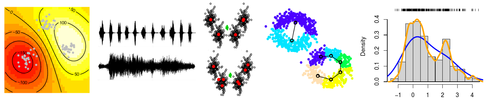
\includegraphics[width=9cm]{img/mi2}
\end{center}

``interesting'' and  ''structure'' is expressed through the objective model.

\end{frame}

\begin{frame}{\subsubsecname}

\underline{Data}:

A dataset of observations:
\begin{equation}
\label{eq:observations}
\vec X = 
\left(
\begin{array}{cccccc}
\Big| & \Big| & & \Big| & & \Big| \\[3mm]
\vec x^{(1)} & \vec x^{(2)} & \cdots & \vec x^{(\alpha)} & \cdots & \vec x^{(p)}\\[2mm]
\Big| & \Big| & & \Big| & & \Big|
\end{array}
\right) \in \R^{N \times p}
\end{equation}
\notesonly{
where $p$ denotes the number of observations (i.e. size of the dataset) and $N$ denotes the number of dimensions.}
\slidesonly{
where 
\begin{itemize}
\item[] $p$ \corresponds\, no. of observations (often \iid)
\item[] $N$ \corresponds\, no. of dimensions
\end{itemize}
}
\notesonly{
The samples are often assumed to be \iid, but algorithms for handling sequential data also exist.

Example: $\vec x$ could represent user ratings, pixel values in images.
}
\end{frame}
\begin{frame}

\underline{Objective model}:
\mode<presentation>{\vspace{5mm}}
\mode<article>{
An unsupervised learning algorithm is used to capture structure or directions in the data. This can be achieved by finding:
}
\begin{itemize}
\item the underlying distribution $P(\vec x)$ that generated this data (e.g. density estimation),
\item $\vec z := \vec f(\vec x)$, where $\vec z$ is a measure of 
\begin{itemize}
\item possible structure such as clustering or grouping in the data ($\vec z \in {0,\ldots,K-1}$), \\

and/or

\item possible directions in the data, by finding another continuous space for describing this data. \\

Example: dimensionality reduction, $\vec z \in \R^M$ with $M < N$.

\end{itemize}
\end{itemize}

\end{frame}

\mode*

\clearpage

\mode<all>
\section{Precursor: Method of Lagrange Multipliers}

\definecolor{darkgreen}{rgb}{0,0.6,0}

\begin{frame}
	\slidesonly{
	\begin{center}\Large
	\secname
	\end{center}
	\pause
	}
    \begin{center}
    \slidesonly{\huge}
	Don't panic!
    \end{center}
    \begin{center}
        Essentially just hill-climbing (gradient ascent)
    \end{center}
    \pause

\underline{Objective}: \\
\textit{Maximize} an objective function while also satisfying some constraint(s).\\
{
\small(\textit{Maximize}: Find the arguments that maximize an objective function.)
}\\

Don't forget: any maximization problem can be turned into a minimization problem\notesonly{ by maximizing the ``negative'' of the function}.
\end{frame}

\subsection{Gradient ascent - unconstrained optimization}
\begin{frame}\frametitle{\subsecname}
Maximize an objective function $f(w_1, w_2)$ (no constraints here).\\
Here $w_1$ and $w_2$ are referred to as free parameters.\\

\begin{figure}[h]
	\centering
	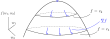
\includegraphics[width=0.8\linewidth]{img/lagrange_objfunction}%
	\notesonly{
	\caption{
	An unconstrained optimization problem.
	}%
	}%
    \label{fig:unconstrained}%
\end{figure}

\mode<article>{
\figref{fig:unconstrained} depicts the objective function $f$ we want to maximize (i.e. reach the blue $\color{blue}\times$ at the top). $c_1$ and $c_2$ are level curves where $f$ is constant. 
	The blue arrows indicate the direction of the gradient $\vec \nabla f$, which is always perpendicular to the level curve.
}

\slidesonly{
\vspace{-3mm}
}

The gradient $\vec \nabla f$ describes the direction of greatest ascent:\\
\slidesonly{
\vspace{-3mm}
}
\begin{equation}
\vec \nabla f = 
\frac{\partial f}{\partial \vec w} = 
\rmat{\frac{\partial f}{\partial w_1} \\[0.2cm] \frac{\partial f}{\partial w_1} }
\end{equation}

\end{frame}

\subsection{Adding a single constraint}

\begin{frame}\frametitle{\subsecname}
We restrict solutions to those that satisfy the constraint $g(w_1, w_2) = c$:

\begin{figure}[h]
\centering
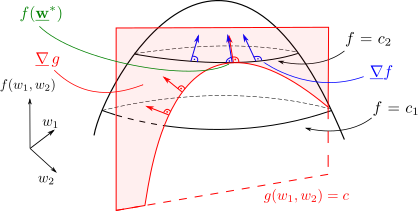
\includegraphics[width=0.7\linewidth]{img/lagrange_objfunction_constrained}
\mode<article>{
\caption{The surface of the constraint cuts through the surface of the objective function. The highest point that can be reached on $f$ which also intersects with $g$ is unique in that the gradients of $f$ and $g$ both point in the same direction with only a difference in scale.}
}
\end{figure}

\only<1,2>{
\question{What is characteristic of the solution ${\color{darkgreen}\vec w^{*}}$ to the constrained optimization problem?}\\
}
\notesonly{
-The solution of the constrained optimization problem is characterized by:
}
\only<2>{
\slidesonly{\vspace{-5mm}}
\begin{equation}
    \vec \nabla f \big|_{\color{darkgreen}\vec w^{*}} = \lambda' \vec \nabla g\big|_{\color{darkgreen}\vec w^{*}} \,,\quad
\text{where $\lambda'$ is a scaling factor.}
\label{eq:equality}
\end{equation}
}
\notesonly{\eqref{eq:equality} holds for the highest position in $f$ while also satisfying the constraint.\\

Consequently,}
% temporarily change footnote marks to symbols so not to confuse with exponents
\renewcommand*{\thefootnote}{\fnsymbol{footnote}}
\only<3>{
\slidesonly{\vspace{-5mm}}
\begin{align}
  \vec \nabla f \; - \lambda' \vec \nabla g     &= \vec 0 \\
  \vec \nabla f \; + \underbrace{(- \lambda')}_{=:\lambda} \vec \nabla g &= \vec 0 \\
  \vec \nabla f \;  + \lambda \vec \nabla g      &= \vec 0\notesonly{\;\footnotemark }
  \label{eq:equalitylambda}
\end{align}
}
\notesonly{
    \footnotetext{
    The switch from $\lambda'$ to $\lambda$ is to be more consistent with the lecture slides.
    }
}
% change footnote marks back to original scheme (numbers)
\renewcommand*{\thefootnote}{\arabic{footnote}}

\end{frame}

\begin{frame}
\only<1,2>{
The constrained optimization problem is formulated as:
\begin{equation}
\underbrace{f(w_1, w_2) \;\eqexcl\; \max_{w_{1},w_{2}}}_{\text{maximization}} \quad  \text{subject to} \quad \underbrace{g(w_1,w_2)\;-c\; = \; 0}_{\text{a single constraint}}
\label{eq:optconstrained}
\end{equation}
}
\notesonly{
The \emph{Lagrangian} function reformulates the constrained optimization problem from \eqref{eq:optconstrained} in a way that reflects the relationship of the two gradients at the solution and thus facilitate finding the solution \eqref{eq:equalitylambda}.} The \emph{Lagrangian} is \notesonly{therefore }defined as:

\only<2,3>{
\begin{equation}
L(w_1, w_2, \lambda) \; := \; f(w_1,w_2) + \lambda\big(g(w_1, w_2)-c\big)
\end{equation}

Setting the gradient $\nabla L$ to zero guarantees a solution at which $\vec \nabla f \;  + \lambda \vec \nabla g = \vec 0$
}
\only<3>{

\begin{equation}
\vec \nabla L = 
\rmat{
	\frac{\partial L}{\partial w_1} \\[0.5cm]
	\frac{\partial L}{\partial w_2} \\[0.5cm]
	\frac{\partial L}{\partial \lambda}
	}
=
\rmat{
	\;\frac{\partial f}{\partial w_1} \quad\;\;+\quad\;\; \lambda \frac{\partial g}{\partial w_1} \;\\[0.3cm]
	\;\frac{\partial f}{\partial w_2} \quad\;\;+\quad\;\; \lambda \frac{\partial g}{\partial w_2} \;\\[0.3cm]
	\underbrace{\frac{\partial f}{\partial \lambda}}_{=0} \;+\quad g(w_1, w_2)-c
	}
=
\rmat{
	0 \\[0.5cm]
	0 \\[0.5cm]
    0
	}
= \vec 0
\label{eq:lagrangiangrad}
\end{equation}

Setting the first two elements of $\vec \nabla L$\notesonly{, namely $\frac{\partial L}{\partial w_1}$ and $\frac{\partial L}{\partial w_2}$,} to zero ensures that $\nabla f = -\lambda \nabla g$,\\
while $\frac{\partial L}{\partial \lambda}=0$ ensures that $g(w_1, w_2) = c$.\\

\notesonly{\eqref{eq:lagrangiangrad} describes a system of }3 equations with 3 unknowns.\notesonly{
\footnote{
Not much emphasis is put on knowing how to solve this by hand. If interested, the Wikipedia article on \href{https://en.wikipedia.org/wiki/Lagrange_multiplier\#Examples}{Lagrange multiplier} provides some examples.}
}\\

We refer to $\lambda$ as the \emph{multiplier} for the constraint $c$.
}
\end{frame}

\newpage

\subsection{Multiple constraints}

\begin{frame}
 
\question{How do we extend this to multiple {\color{red}{equality}} constraints?}

\slidesonly{\vspace{-2mm}}
    
\begin{equation}
\underbrace{f_0(\vec w) \;\eqexcl\; \text{max}}_{\text{maximization}} \quad  \text{and} \quad f_k(\vec w)\;{\color{red}{=}}\; \; 0 \;, \quad k = 1,\ldots,m
\label{eq:optimizationequalitymultipe}
\end{equation}

where $m$ denotes the number of constraints. $f_{0}(\vec w)$ is reserved for the function to be optimized., while $f_{1}(\vec w), f_{2}(\vec w),\ldots,f_{m}(\vec w)$ is used for all $m$ constraints.

The Lagrangian for multiple constraints is defined as:
%\slidesonly{\vspace{-2mm}}
\begin{align}
L(\,\vec w\;, \overbrace{\{\lambda_k\}}^{
\mathclap{
\substack{\text{a multiplier} \\
\text{for each constraint}}
}
}) 
\; :=& \; 
f_0(\vec w) + \lambda_1 \, f_1(\vec w) + \lambda_2 \, f_2(\vec w) + \, \ldots \, + \lambda_m \, f_m(\vec w) \\
\; =& \; 
f_0(\vec w) + \sum_{k=1}^{m} \lambda_k \, f_k(\vec w)
\label{eq:lagrangianmultiple}
\end{align}

\question{What if we have {inequality} constraints?}

\end{frame}

\begin{frame}

In the case of {\color{red}{inequality}} constraints, our constrained optimization problem would have the following form:

\begin{equation}
\underbrace{f_0(\vec w) \;\eqexcl\; \text{max}}_{\text{maximization}} \quad  \text{and} \quad f_k(\vec w)\; {\color{red}{\le}} \; 0 \;, \quad k = 1,\ldots,m{}
\label{eq:optimizationINequalitymultipe}
\end{equation}

However, the Lagrangian remains the same\notesonly{ as in \eqref{eq:lagrangianmultiple}}. The inequality is taken into account in that the solutions for $\lambda$ extend to some range:

\begin{equation}
L(\,\vec w\;, \{\lambda_k\}
) \; := \; f_0(\vec w) + \sum_{k=1}^{m} \lambda_k \, f_k(\vec w)\,,\qquad
\lambda_{k} \;{\color{red}{\ge}}\; 0 \quad \forall k \in \{1,\ldots,m\}
\label{eq:lagrangianINequalitymultiple}
\end{equation}
 
    
\end{frame}

\mode*

\clearpage

%\section{References}
%\begin{frame}[allowframebreaks] \frametitle{References}
	%\scriptsize
	%\bibliographystyle{plainnat}
	%\bibliography{bibliography}
%\end{frame}

\end{rightcolumn}
\end{paracol}

\end{document}
